%!TeX spellcheck = en-GB

%Basics
\documentclass[aps, prb, a4paper, english, 12pt, onecolumn, longbibliography, amsmath, amssymb, colorinlistoftodos, floatfix, svgnames]{revtex4-2}
\usepackage[utf8]{inputenc}
\usepackage{babel}

%Symbols and scientifics
\usepackage{amsmath, amsfonts, amssymb, bm}
\numberwithin{equation}{subsection}
\usepackage{physics}
\usepackage{mathtools}
\usepackage{siunitx}
\sisetup{
	per-mode = power ,
	round-mode = figures ,
	round-precision = 3 ,
	scientific-notation = false ,
	output-decimal-marker = {.} ,
	exponent-product = \times ,
	separate-uncertainty = true ,
	uncertainty-separator = \ ,
	output-product = \cdot ,
	quotient-mode = fraction ,
	range-phrase = - ,
	range-units =  single ,
	inter-unit-product = \ensuremath{{\cdot{}}} ,
	number-unit-product = \ ,
	multi-part-units = single ,
	alsoload = synchem ,
	alsoload = addn
}
\DeclareSIUnit\atm{atm}
\usepackage{chemfig}
\usepackage{tikzorbital}

%Appendix, TOC and Bibliography
\usepackage{appendix}
\renewcommand\appendixtocname{Appendices}
%\usepackage[nottoc]{tocbibind}
\usepackage[lastpage,user]{zref}

%Figures
\usepackage{float}
\usepackage{xcolor} % Required to specify font color
\usepackage{graphicx}
\usepackage{subcaption}
\usepackage[format=plain,
            labelfont={bf,it},
            textfont=it]{caption}
\usepackage[verbose]{wrapfig}
\usepackage[a4paper, centering, rmargin=2.5cm, tmargin=2.5cm, lmargin=2.5cm, bmargin=2.5cm]{geometry}
\usepackage{etoolbox}
\usepackage{verbatim}
\usepackage[space]{grffile}
\usepackage[final]{pdfpages}
\usepackage{array}
\usepackage{multirow}
\usepackage{dcolumn}
%\usepackage{animate}
\usepackage{fontawesome}
\usepackage[european]{circuitikz}
\usepackage{pdflscape}
\usepackage{pgfplots}
\pgfplotsset{width=10cm, compat=newest}
\def\axisdefaultwidth{10cm}
%\usepgfplotslibrary{external}
\usepgfplotslibrary{units}
%\tikzexternalize
\usepackage{pgfgantt}
\newcounter{myWeekNum}
\stepcounter{myWeekNum}
%
\newcommand{\myWeek}{\themyWeekNum
    \stepcounter{myWeekNum}
    \ifnum\themyWeekNum=53
         \setcounter{myWeekNum}{1}
    \else\fi
}
%

%Header footer
\usepackage{fancyhdr}
\pagestyle{fancy}
\lhead{C. V. Sørensen \\ R. K. F. Wiuff}
\chead{Quantum Transport in NPG\\DTU Department of Physics}
\rhead{May \nth{1}\\2019}
\cfoot{Page \thepage\, of \zpageref{LastPage}}
\renewcommand{\headrulewidth}{0.4pt}
\renewcommand{\footrulewidth}{0.4pt}

%Text tools
\usepackage[super]{nth}
\usepackage[normalem]{ulem}
\usepackage{import}
\usepackage{url}
\usepackage{lipsum}
\usepackage{microtype}
\usepackage[pdfencoding=auto, psdextra]{hyperref}
\hypersetup{
	colorlinks   = true, %Colours links instead of ugly boxes
	urlcolor     = blue, %Colour for external hyperlinks
	linkcolor    = blue, %Colour of internal links
	citecolor   = red %Colour of citations
}
\usepackage[capitalise]{cleveref}
\usepackage{enumitem}
\setlist[enumerate]{itemsep=0mm}
\usepackage{booktabs}
\usepackage{silence}
\usepackage{todonotes}
\WarningFilter{revtex4-2}{Repair the float package.}

%Python
\usepackage{minted}
\setminted{fontsize=\small}
\usemintedstyle{monokai}
\renewcommand{\listoflistingscaption}{Listings}
%\renewcommand{\MintedPygmentize}{C:/Users/rwiuf/AppData/Roaming/Python/Python37/Scripts/pygmentize}
\newcommand{\im}[2]{\inputminted[bgcolor=Black,linenos=true]{#1}{#2}}

%Definitions and new commands
\newcommand{\degr}{^{\circ}}
\newcommand{\me}{\mathrm{e}}
\newcommand*\mathinhead[2]{\texorpdfstring{$\boldsymbol{#1}$}{#2}}
%PDFPages and RevTeX incompatability fix
\makeatletter
\AtBeginDocument{\let\LS@rot\@undefined}
\makeatother

\begin{document}
%Titlepage herunder:
\begin{abstract}
	\vspace{5mm}
	\centering
	\begin{description}
		\item[Abstract] Abstract... \vspace{3\baselineskip}
	\end{description}
	
\includegraphics[width=1cm]{Figures/DTU3CMYK.eps}
\end{abstract}

\title{Quantum Transport in Nanoporous Graphene}
\date{May \nth{1} 2019}
\author{Rasmus Kronborg Finnemann Wiuff (s163977)}
\email[E-mail at ]{rwiuff@dtu.dk}
\author{Christoffer Vendelbo Sørensen (163965)}
\email[E-mail at ]{chves@dtu.dk}
\affiliation{Technical University of Denmark}
\homepage[Homepage of the Technical University of Denmark ]{http://www.dtu.dk/english/}
\homepage[\\\faGithub \ Project Repository: ]{https://github.com/rwiuff/QuantumTransport}
\maketitle

\pagenumbering{arabic}

\tableofcontents

% ToC before List-ofs fix
\makeatletter
\let\toc@pre\relax
\let\toc@post\relax
\makeatother

\thispagestyle{empty}
%\newpage
\setcounter{page}{1}

%Text
\subsection{Intro}
%!TEX root = ../Main.tex
\lipsum{5}\cite{calogero_electron_2019}
\subsection{Pi-orbitals and Basis sets }
\newpage
\begin{acknowledgments}
	The authors would like to thank...
\end{acknowledgments}
%End of text
% List of ToDos
%\listoftodos %Uncomment for list of todos
%Bibliography herunder:
%\newpage
\onecolumngrid
\bibliography{Bibliography}

\newpage
\listoffigures
\listoftables
\listoflistings
%\listoftodos
\newpage
 %Appendicer herunder:
% !TEX root = Main.tex
\appendix
\appendixpage
\addappheadtotoc
\section{Additional figures}\label{appfigs}
\begin{figure}[h]
	\centering
	\begin{subfigure}[b]{0.3\textwidth}
		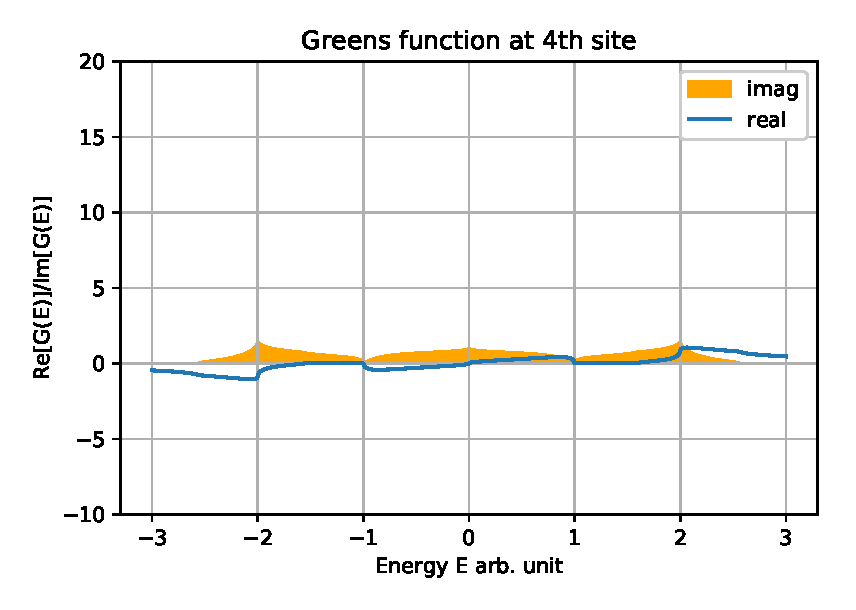
\includegraphics[width=\textwidth]{Figures/BetaimrealTE4.eps}
		\caption{Figure showing a plot of the Green's function at the 4th site}
		\label{4th}
	\end{subfigure}
	~ %add desired spacing between images, e. g. ~, \quad, \qquad, \hfill etc.
	%(or a blank line to force the subfigure onto a new line)
	\begin{subfigure}[b]{0.3\textwidth}
		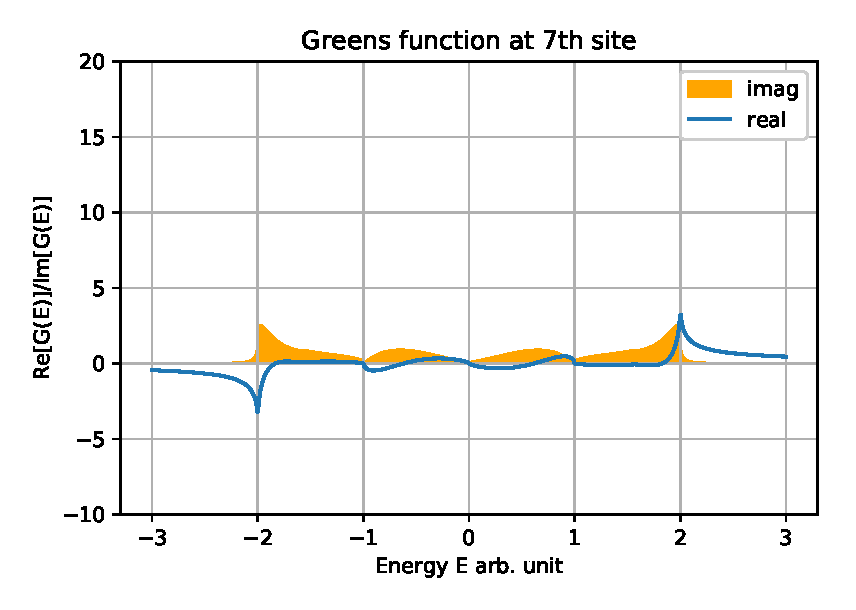
\includegraphics[width=\textwidth]{Figures/BetaimrealTE7.eps}
		\caption{Figure showing a plot of the Green's function at the 7th site}
		\label{7th}
	\end{subfigure}
	\caption{Two plots showing how the Green's function changes as the site is changed. The 4th and 7th sites are corresponding to atoms of those indices (4, 7) in \cref{pointplot}. Note how the LDOS changes (imaginary part) for the different sites.}\label{siteLDOSplot}
\end{figure}
\begin{figure}
	\centering
	\begin{subfigure}[b]{0.3\textwidth}
		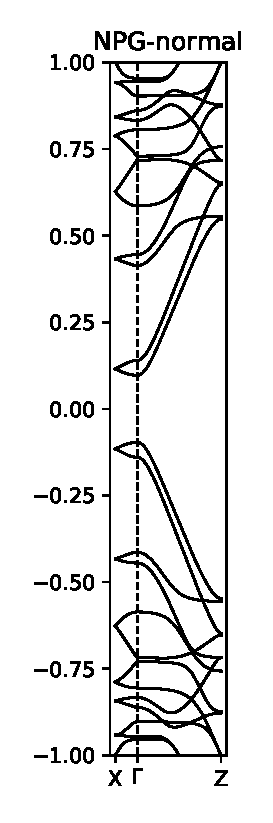
\includegraphics[width=\textwidth]{Figures/FabNPGBS.eps}
		\caption{Plot showing the band structure in the energy range \SI{-1.5}{\electronvolt} to \SI{1.5}{\electronvolt} for NPG with normal bridges between symmetry points \(X\) and \(Y\) with respect to \(\Gamma\)}
		\label{Fabbs}
	\end{subfigure}
	~ %add desired spacing between images, e. g. ~, \quad, \qquad, \hfill etc.
	%(or a blank line to force the subfigure onto a new line)
	\begin{subfigure}[b]{0.3\textwidth}
		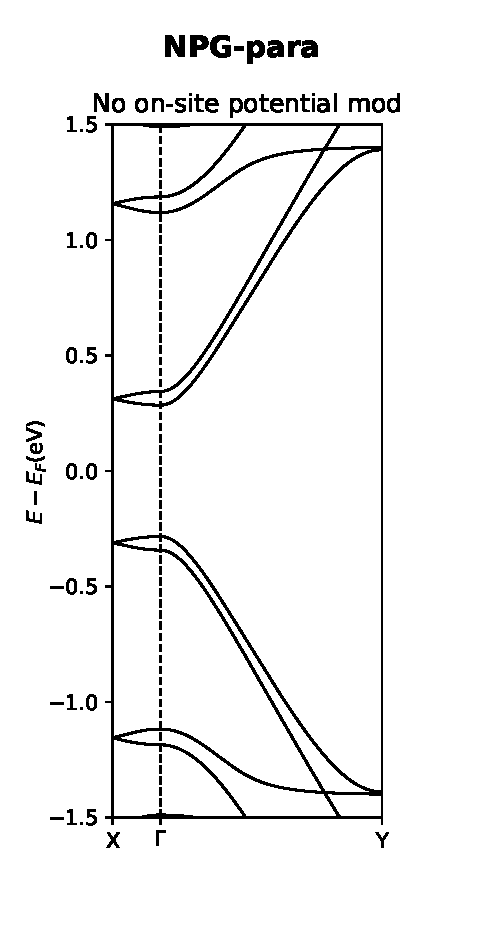
\includegraphics[width=\textwidth]{Figures/paraNPGBS.eps}
		\caption{Plot showing the band structure in the energy range \SI{-1.5}{\electronvolt} to \SI{1.5}{\electronvolt} for NPG with para bridges between symmetry points \(X\) and \(Y\) with respect to \(\Gamma\)}
		\label{parabs}
	\end{subfigure}
	~ %add desired spacing between images, e. g. ~, \quad, \qquad, \hfill etc.
	%(or a blank line to force the subfigure onto a new line)
	\begin{subfigure}[b]{0.3\textwidth}
		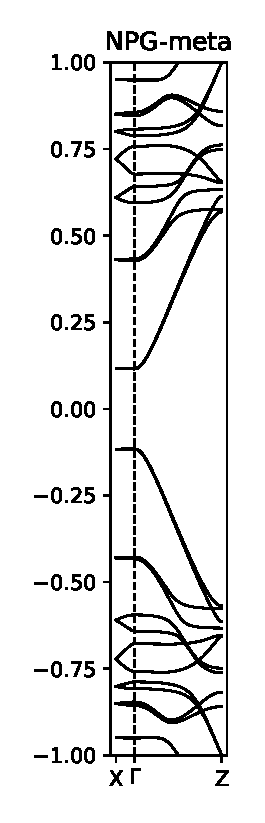
\includegraphics[width=\textwidth]{Figures/metaNPGBS.eps}
		\caption{Plot showing the band structure in the energy range \SI{-1.5}{\electronvolt} to \SI{1.5}{\electronvolt} for NPG with meta bridges between symmetry points \(X\) and \(Y\) with respect to \(\Gamma\)}
		\label{metabs}
	\end{subfigure}
	\caption{Figure showing para, meta and normal NPG band structures}\label{allbands}
\end{figure}
\im{Listings/Functions.py}{41}{47}
\vspace{-1\baselineskip}
\captionof{listing}{Function creating the hopping matrices between two sets of coordinates \label{hopfunc}}\vspace{\baselineskip}

\begin{figure}
	\centering
	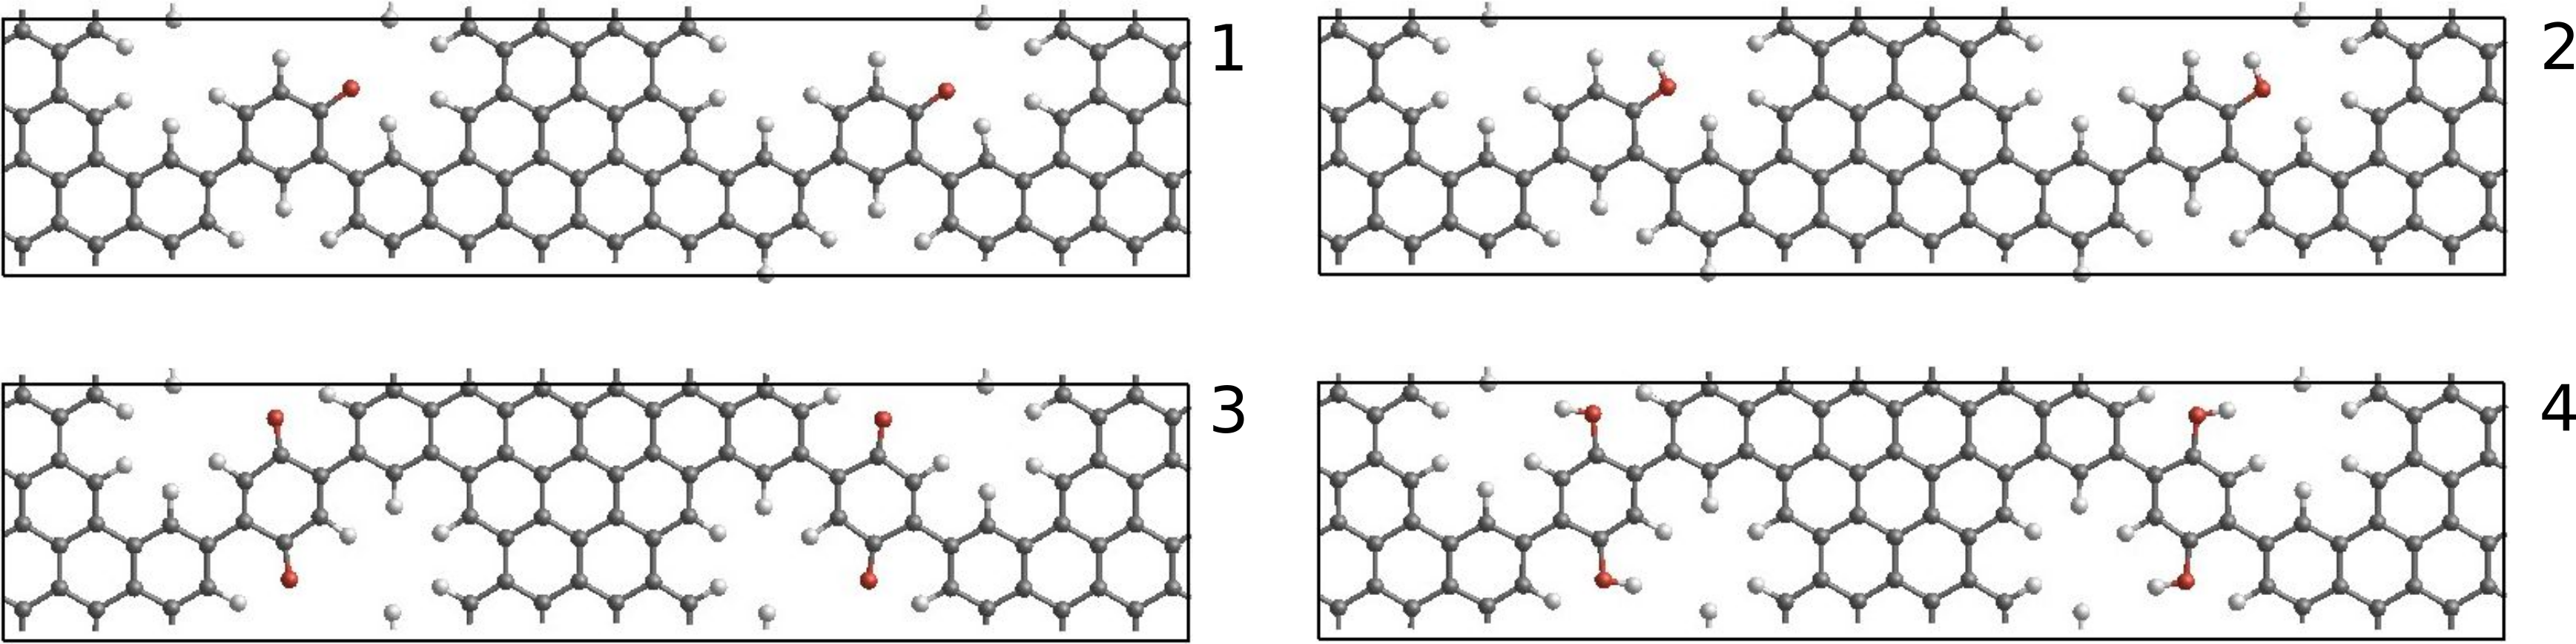
\includegraphics[width=\textwidth]{Figures/Structures.png}
	\caption{Figure showing all the structures stated in \cref{testtable}.}
	\label{Strucow}
\end{figure}

\im{Listings/Functions.py}{245}{252}
\vspace{-1\baselineskip}
\captionof{listing}{Code piece showing how the periodic Hamiltonian, shifted in the transverse direction i created using the given unit vector in the y direction.}{\label{periodichamilcode}}\vspace{\baselineskip}

\im{Listings/Functions.py}{234}{242}
\vspace{-1\baselineskip}
\captionof{listing}{Code piece showing how the transmission per energy point, using equation \cref{}.}{\label{transmissioncode}}\vspace{\baselineskip}

% \section{Project overview}
% A Gantt chart is provided on the next page. \textbf{Not Updated.}
% \newpage
% \begin{turnpage}
% \setcounter{myWeekNum}{6}
% \ganttset{%
% 	calendar week text={\myWeek{}}%
% }
% \begin{figure}\vspace{-10mm}
% \begin{ganttchart}[
% 		hgrid,
% 		vgrid={*{6}{draw=none}, dotted},
% 		x unit=.15cm,
% 		%	y unit title=.6cm,
% 		%	y unit chart=.6cm,
% 		inline,
% 		milestone inline label node/.append style={left=5mm},
% 		milestone/.append style={xscale=3},
% 		time slot format=isodate,
% 		time slot format/start date=2019-02-04
% 	]{2019-02-04}{2019-05-31}
% 	\gantttitlecalendar{year, month=shortname, week}\\
% 	\ganttgroup{Report writing}{2019-02-25}{2019-05-31}\\
% 	\ganttgroup[inline = false]{Course 33442}{2019-02-04}{2019-03-31}\\
% 	\ganttbar{Ch. 1 \& 2}{2019-02-04}{2019-02-17}\\
% 	\ganttlinkedbar[link bulge=2]{Ch. 3}{2019-02-18}{2019-02-24}\\
% 	\ganttlinkedbar[link bulge=2,bar inline label node/.style={right=15pt}]{Ch. 4 \& 5}{2019-02-25}{2019-03-03}\\
% 	\ganttgroup[inline = false]{Python code}{2019-03-04}{2019-03-31}\\
% 	\ganttbar{Py TB scripts}{2019-02-18}{2019-03-17}\\
% 	\ganttlinkedbar[link bulge=2, bar inline label node/.style={right=45pt}]{Small NPG systems simulations}{2019-03-10}{2019-03-31}\\
% 	\ganttmilestone{Proof of Concept with Python}{2019-03-31}\\
% 	\ganttgroup[inline = false]{Large scale TB}{2019-04-01}{2019-04-28}\\
% 	\ganttbar[bar inline label node/.style={left=10pt}]{SISL \& TBtrans tutorial}{2019-04-01}{2019-04-05}\\
% 	\ganttlinkedbar[link bulge=2, bar inline label node/.style={right=50pt}]{Setup NPG variations}{2019-04-06}{2019-04-28}\\
% 	\ganttgroup[inline = false]{Generate data}{2019-04-28}{2019-05-31}\\
% 	\ganttmilestone{Hand in report}{2019-05-31}
% \end{ganttchart}
% \end{figure}
% \end{turnpage}
% \clearpage
% \global\pdfpageattr\expandafter{\the\pdfpageattr/Rotate 90}

\end{document}
